\documentclass[french, 12pt, a4paper, onesided]{scrartcl}
\usepackage[T1]{fontenc} %font (Umlaute)
\usepackage[utf8]{inputenc} %font
\usepackage{mathptmx} %Font Times
\usepackage{lmodern} %Font Latin Modern
\usepackage{amsthm} %Defininig Theorems
\usepackage{amsmath} %Mathematical Extention for LaTeX
\usepackage{amsfonts} %Mathematical Fonts
\usepackage{amssymb} %Mathematical Symbols
\usepackage[left=2.60cm, right=2.60cm, top=2.80cm, bottom=3.40cm]{geometry} %Preferences: Page
\usepackage[ngerman,german,english]{babel} %Language (Umlaute)
\usepackage{paralist} %Preferences for Enumeration
\usepackage{titlesec} %Preferences for Sections
\usepackage[titles]{tocloft} %Preferences for Table of Contents
\usepackage{graphicx} %Including Graphics
\usepackage{epstopdf} %allows including in pdfs
\usepackage{caption}  %für die nutzung von subfigures
\usepackage{subcaption} %für die nutzung von subfigures




%%%%%%%%%%%%%%%%% Section Preferences %%%%%%%%%%%%%%%%%

\titleformat{\section}[block]{\normalsize\centering\scshape}{\thesection.}{4pt}{}{}
\titlespacing{\section}{0pt}{25pt}{12pt}[0pt]


%%%%%%%%%%%%%%% Theormstyles and Definition %%%%%%%%%%%%%%%

\renewcommand{\labelenumi}{(\alph{enumi})} %default style for enumeration: (a), (b), (c)

\theoremstyle{plain}
\newtheorem{thm}{Theorem}[section]
\newtheorem{cor}[thm]{Corollary}
\newtheorem{lem}[thm]{Lemma}
\newtheorem{pro}[thm]{Proposition}

\theoremstyle{definition}
\newtheorem{defi}[thm]{Definition}
\newtheorem{rem}[thm]{Remark}

\theoremstyle{remark}
\newtheorem{exa}[thm]{Example}

%%%%%%%%%%%%%%%%%%%%  Macros  %%%%%%%%%%%%%%%%%%%%

\newcommand{\C}{\mathbb{C}}
\newcommand{\N}{\mathbb{N}}
\newcommand{\Q}{\mathbb{Q}}
\newcommand{\R}{\mathbb{R}}
\newcommand{\rimp}{\;\Longrightarrow\;}
\newcommand{\limp}{\;\Longleftarrow\;}
\newcommand{\lrimp}{\;\Longleftrightarrow\;}

\newcommand{\T}{\text{T}}
\newcommand{\ve}[1]{{\emph{\textbf{#1}}}}
\newcommand{\norm}[2][]{\left\|#2\right\|_{#1}}
\newcommand{\dist}[2]{\textup{dist}\left(#1,#2\right)}
\newcommand{\skp}[2]{\left\langle #1,#2 \right\rangle}

%%%%%%%%%%%%%%%%% Title/Author/Date %%%%%%%%%%%%%%%%%

\title{\textrm{\textbf{\large Numerik Projekt 1 -- Aufgabe 1}}}

\author{\normalsize Lukas Moser \& Bernhard Kepka}

\date{}


%%%%%%%%%%%%%%%%%% ------ Document ------ %%%%%%%%%%%%%%%%%%

\begin{document}

\begin{minipage}[t]{\textwidth}
	\vspace*{-6.7\baselineskip}
	\maketitle
\end{minipage}
\vspace{-1.0cm}

\section{Gauß-Quadratur auf $ [-1,1] $}
Die zur Gauß-Quadratur auf dem Intervall $ [-1,1] $ mit der Gewichtsfunktion $ w\equiv1 $ gehörenden (normierten) Orthogonalpolynome sind durch die Legendre-Polynome $ L_j $ gegeben. Letztere erfüllen die Rekursion
\begin{align}\label{eq:Lrek}
	L_0(x)=1, \quad L_1(x)=1 \quad L_{n+1}(x)=xL_n(x)-\frac{n^2}{4n^2-1}L_{n-1}(x), \; n\in\N.
\end{align}
Da das gegeben Intervall und die Gewichtsfunktion symmetrisch sind, folgt für die $ n+1 $ Knoten $ (x_j) $ und Gewichte $ (\alpha_j) $ (nach einem Übungsbeispiel) $ x_j=-x_{n-j} $ beziehungsweise $ \alpha_j=\alpha_{n-j} $ für $ j=0,\ldots, n $.
\newline
Zur konkreten Implementierung wurden zwei Weg verfolgt:
\begin{enumerate}[(i)]
	\item Die Quadraturknoten wurden gemäß Satz 4.23 des Numerik-Skriptums über eine Eigenwertaufgabe und die Quadraturgewichte über entsprechende Eigenvektoren berechnet.
	\item Über die rekursive Darstellung der Legendre-Polynome lassen sich örtliche Beziehungen zwischen Nullstellen zweier Polynome $ L_n $ und $ L_{n+1} $ extrahieren. Mittels bekannter Nullstellen des $ n $-ten Polynomes und eines Sekanten-Verfahrens wurden in Folge die Nullstellen von $ L_{n+1} $ ermittelt.
\end{enumerate}
In beiden Fällen können die Gewichte mit Hilfe der Nullstellen von $ L_{n+1} $ und der Legendre-Polynome $ L_0,\ldots,L_n $ explizit angegeben werden.

\paragraph{1. Via Eigenwertaufgabe.} Mit Satz 4.23 und obiger 3-Term-Rekursion folgt (Bezeichnungen wie im Satz) $ \gamma_n^2=\frac{n^2}{4n^2-1} $ und $ \beta_n=0 $, denn $ L_{n+1}(X)=\det(IX-T) $. Damit hat die entsprechende Matrix $ T $ die Form
\begin{align*}
	T=\left( \begin{array}{ccccc}
	0 & \gamma_1 &  &  &  \\ 
	\gamma_1 & 0 & \gamma_2 &  &  \\ 
	& \gamma_2 & \ddots & \ddots &  \\ 
	&  & \ddots & \ddots & \gamma_n \\ 
	&  &  & \gamma_n & 0
	\end{array} \right) \in \R^{(n+1)\times(n+1)}.
\end{align*}
Die Nullstellen von $ L_{n+1} $ sind entsprechend die Eigenwerte von $ T $. Für die Gewichte gilt die Beziehung
\begin{align}
	\alpha_j=\left( \dfrac{(v_j)_1}{\norm[2]{v_j}} \right)^2 \int_{-1}^1w(x)dx=2\left( \dfrac{(v_j)_1}{\norm[2]{v_j}} \right)^2,
\end{align}
wobei $ (v_j)_1 $ die 1. Komponente eines Eigenvektors $ v_j $ von $ T $ ist.
\newline
Mit den internen Funktionen von Matlab wurden nun die Eigenwerte bzw. Eigenvektoren berechnet.

\paragraph{2. Rekursive Knotenberechnung.} Wegen der Symmetrie um den Ursprung genügt es die positiven Nullstellen zu betrachten. Für ungerades $ n $ ist $ 0 $ stets ein Quadraturknoten.
\newline
Wir nutzen nun folgende Eigenschaften zur besseren Bestimmung der Nullstellen.
\begin{itemize}
	\item Für die Nullstellen der Legendre-Polynome $ L_1,\ldots,L_n $ gilt: Zwischen je zwei positiven Nullstellen von $ L_{n-1} $ befindet sich genau eine von $ L_n $.
	\newline
	Dies sieht man induktiv ein: für $ n=1,2,3 $ gilt die Aussage durch die entsprechenden Nullstellen. Seien nun $ x^{(n)},y^{(n)} $ zwei Nullstellen von $ L_n $. Nach Induktionsannahme befindet sich eine Nullstelle $ z^{(n-1)} $ von $ L_{n-1} $ in $ (x^{(n)},y^{(n)}) $. Da $ z^{(n-1)} $ einfach ist, hat $ L_{n-1} $ einen Vorzeichenwechsel in diesem Intervall. $ xL_n(x) $ hat konstantes Vorzeichen. Wegen \eqref{eq:Lrek} folgt also, dass das Vorzeichen von $ L_{n+1} $ in den Randpunkten (beziehungsweise in einer Umgebung von diesen) alleine von $ L_{n-1} $ bestimmt wird. Aus dem Zwischenwertsatz folgt, dass sich eine Nullstelle in $ (x^{(n)},y^{(n)}) $ befindet. Da $ L_{n-1} $ genau einmal sein Signum wechselt, kann es nur genau eine sein.
	\item Nun folgt: es gibt eine Nullstelle von $ L_n $, die größer ist als alle von $ L_{n-1} $.
	\\
	Für $ n=1,2,3,4,5 $ gilt dies.
	\newline
	Seien $ x_1^{(n-1)},\ldots,x_k^{(n-1)} $ die positiven Nullstellen von $ L_{n-1} $ mit $ k=\lfloor \frac{n}{2}\rfloor $. In den Intervallen $ (x_1^{(n-1)},x_2^{(n-1)}),\ldots,(x_{k-1}^{(n-1)},x_k^{(n-1)}) $ befinden sich genau eine Nullstelle von $ L_n $, also $ \lfloor \frac{n}{2}\rfloor-1 $. Ist $ n $ ungerade, so ist $ 0 $ eine weiter und wir haben $ n-2 $ Nullstellen in $ (-1,1) $ gefunden. Die letzten zwei müssen sich ebenfalls in diesem Intervall befinden. Da sie nicht mit $ \pm x_k^{(n-1)} $ übereinstimmen, befinden sie sich in den Intervallen $ (-1,-x_k^{(n-1)})  $ und $ (x_k^{(n-1)},1) $. Wegen der Symmetrie folgt die Behauptung.
\end{itemize}
Darauf aufbauend führt man bei bekannten (positiven) Nullstellen von $ L_n $ ein Sekantenverfahren zwischen aufeinanderfolgende durch. Zusätzlich macht man selbiges mit dem Intervall $ (x_k^{(n)},1) $, wobei $ x_k^{(n)} $ die größte Nullstelle von $ L_n $sei. Je nachdem, ob $ n $ gerade oder ungerade ist, muss man noch ein Sekantenverfahren zwischen Null und der kleinsten Nullstelle durchführen oder Null selbst als Knoten wählen.

\paragraph{3. Explizite Darstellung der Gewichte.} Ein Eigenvektor $ v_k $ zum Eigenwert $ x_k $ von $ T \in \R^{(n+1)\times(n+1)} $ hat die Form $ (c_0L_0(x_k),\ldots,c_nL_n(x_k))^T $, wobei $ c_j $ noch zu spezifizierende Konstanten sind. Letztere ergeben sich aus $ Tv_k\stackrel{!}{=}x_kv_k $ durch komponentenweisen Vergleich. Für die erste Zeile gilt
\begin{align*}
	\gamma_1 c_1 L_1(x_k) = \gamma_1c_1 x_k\stackrel{!}{=}x_k c_0 L_0(x_k)=x_kc_0,
\end{align*}
also $ c_1=c_0/\gamma_1 $. Wir setzen $ c_0:=1 $, damit dann $ (v_k)_1=1 $ erfüllt ist. In der $ i $-te Zeile ist mit der Rekursion \eqref{eq:Lrek}
\begin{align*}
	\gamma_{i-1}c_{i-2}L_{i-2}(x_k)+\gamma_ic_iL_i(x_k) &\stackrel{!}{=} x_kc_{i-1}L_{i-1}(x_k) \\
	\iff \gamma_{i-1}c_{i-2}L_{i-2}(x_k)+\gamma_ic_i\left( x_kL_{i-1}(x_k)-\gamma_{i-1}^2L_{i-2}(x_k) \right) &= \\ 
	\left( \gamma_{i-1}c_{i-2}-\gamma_ic_i \gamma_{i-1}^2\right) L_{i-2}(x_k)+\gamma_ic_ix_kL_{i-1}(x_k) &\stackrel{!}{=} x_kc_{i-1}L_{i-1}(x_k).
\end{align*}
Wir haben folglich die Forderungen
\begin{align*}
	\gamma_{i-1}c_{i-2}-\gamma_ic_i \gamma_{i-1}^2 & = 0 \\
	\gamma_ic_i &= c_{i-1}.
\end{align*}
Wenn wir letztere als rekursive Definition von $ c_j $ nutzen, $ c_i:=c_{i-1}/\gamma_i $, gilt auch die erstere
\begin{align*}
	\gamma_i\gamma_{i-1}^2c_i =\gamma_{i-1}^2c_{i-1}=\gamma_{i-1}c_{i-2}.
\end{align*}
Da $ T $ symmetrisch ist und nur einfache Eigenwerte besitzt, sind $ (v_k) $ zueinander orthogonal. Aus der Definition der Quadratur-Formel folgt dann
\begin{align*}
	Q^{(n)}(c_kL_k)=\sum_{i=0}^{n}\alpha_ic_kL_k(x_i)=(c_0L_0,c_kL_k)_w=2\delta_{k0}
\end{align*}
und damit unter Berücksichtigung von $ (v_k)_1=1 $
\begin{align*}
	2=v_k^T2e_1 &= v_k\left(\sum_{j=0}^{n}\alpha_jc_0L_0(x_j),\ldots,\sum_{j=0}^{n}\alpha_jc_nL_n(x_j) \right) ^T = \\
	&= v_k^T\sum_{j=0}^{n}\alpha_jv_j=\alpha_kv_k^Tv_k=\alpha_k\sum_{j=0}^{n}c_j^2L_j(x_k)^2
\end{align*}
Für die Gewichte $ (\alpha_j) $ gilt in Folge
\begin{align}
	\alpha_j=\frac{2}{\sum_{j=0}^{n}c_j^2 L_j(x_k)^2} \qquad j=0,\ldots,n.
\end{align}

\section{Quadratur auf $ [a,b] $ und $ [a,b]\times[c,d] $ }
Mit Hilfe der Transformation
\begin{align*}
	\psi:[-1,1]\rightarrow[a,b]:\xi\mapsto a+\dfrac{b-a}{2}+\xi\dfrac{b-a}{2}=\dfrac{b+a}{2}+\xi\dfrac{b-a}{2}
\end{align*}
wird die Quadratur-Formel aus dem ersten Teil auf $ [a,b] $ übertragen:
\begin{align*}
	\int_{a}^{b}f(x)dx=\int_{-1}^{1}f(\psi(\xi))\left( \dfrac{b-a}{2} \right) d\xi \approx \sum_{j}\left( \dfrac{b-a}{2} \right)\alpha_jf(\psi(x_j)).
\end{align*}
Die Quadratur-Knoten $ (\tilde{x}_j) $ beziehungsweise Gewichte $ (\tilde{\alpha}_j) $ sind also gegeben durch
\begin{align}
	\tilde{x}_j=\psi(x_j)=\dfrac{b+a}{2}+x_j\dfrac{b-a}{2} \qquad \tilde{\alpha}_j=\left( \dfrac{b-a}{2} \right)\alpha_j.
\end{align}
Seien nun zwei Quadraturen $ Q^{(x)} $, $ Q^{(y)} $ auf $ [a,b] $ respektive auf $ [c,d] $ mit Knoten $ (x_i) $, $ (y_j) $  und Gewichten $ (\alpha_i) $, $ (\beta_j) $ gegeben. Auf $ R:=[a,b]\times[c,d] $ folgt mit Fubini
\begin{align*}
	\int_{c}^{d}\int_{a}^{b}f(x,y)dxdy \approx \int_{c}^{d} \sum_{i=1}^{N_x} \alpha_j f(x_i,y)dy = \sum_{i=1}^{N_x} \alpha_j \int_{c}^{d}f(x_i,y)dy \approx \sum_{i=1}^{N_x}\sum_{j=1}^{N_y}\alpha_i \beta_j f(x_i,y_j).
\end{align*}
Jede einzelne Quadratur-Formel ist für Polynome vom Grad $ 2N_x+1 $ bzw. $ 2N_y+1 $ exakt. Für den Funktionenraum $ \Pi_{2N_y+1}^{2N_x+1}:=\left\lbrace p_x(x)p_y(y) \mid  p_x\in\Pi_{2N_x+1}, p_y\in\Pi_{2N_y+1} \right\rbrace  $ ist die Quadratur auf  $ R $ es ebenso:
\begin{align*}
	\int_{a}^{b}\int_{c}^{d}p_x(x)p_y(y)dydx=\int_{a}^{b}p_x(x)Q^{(y)}(p_y)dx=Q^{(x)}(p_x)Q^{(y)}(p_y).
\end{align*}

\paragraph{4. Testen der Implementierung.} Beispiele, a priori Fehlerschätzer (Satz 4.18), Konvergenz (Satz 4.20).
\begin{align*}
	Q(f)-Q_n(f)=\frac{f^{(n+1)}(\xi)}{(2n+2)!}\int_{a}^{b}w(x)\prod_{j=0}^{n}(x-x_j)^2dx 
\end{align*}
\begin{align}\label{eq:apriori1}
	|Q(f)-Q_n(f)|\leq\frac{\norm[\infty]{f^{(n+1)}}}{(2n+2)!}(b-a)^{2n+3}
\end{align}
Für symmetrische Intervalle $ [-c,c] $ erhält man wegen der Symmetrie der Knoten mit
\begin{align*}
	(x-x_j)^2(x-x_{n-j})^2=(x^2-x_j^2)^2\leq c^4\quad \text{also} \\
	|Q(f)-Q_n(f)|\leq 2 \frac{\norm[\infty]{f^{(n+1)}}}{(2n+2)!}c^{2n+3}.
\end{align*}
Genauso kann man aber das Integral folgendermaßen abschätzen:
\begin{align}\label{eq:apriori2}
	\int_{a}^{b}\prod_{j=0}^{n}(x-x_j)^2dx \leq (b-a)^2\int_{a}^{b}\prod_{j=0 , \ j\neq k}^{n}(x-x_j)^2dx=(b-a)^2\alpha_k\prod_{j=0 , \ j\neq k}^{n}(x_k-x_j)^2,
\end{align}
denn es liegt ein Polynom vom Grad $ 2n $ vor. Man wähle $ k $ natürlich so, dass die Differenzen möglichst klein sind. Im Falle symmetrischer Intervalle erhält man
\begin{align*}
	\int_{-c}^{c}\prod_{j=0}^{n}(x-x_j)^2dx \leq 4c^2\alpha_k\prod_{j=0 , \ j\neq k}^{n}x_j^2,
\end{align*}
wenn man schätzungsweise $ x_k=0 $ setzt.

\section{Quadratur auf $ \hat{T} $}
Sei das zweidimensionale Dreieck $ \hat{T}=\text{conv}\{ e_0,e_1,e_2 \} $ mit $ e_0=(0,0)^T $, $ e_1=(1,0)^T $, $ e_2=(0,1)^T $ gegeben. Die Kantenmittelpunkte seien $ k_1=(1/2,0)^T $, $ k_2=(0,1/2)^T $, $ k_2=(1/2,1/2)^T $ und
\begin{align*}
	P_n:=\left\lbrace \sum_{j=0}^{n}\sum_{k=0}^{n-j}a_{jk} x^j y^k \mid a_{jk}\in\R \right\rbrace 
\end{align*} 
der Funktionenraum der Polynome in $ x,y $ mit maximalem Grad $ n $.
\newline
Um Quadraturen $ Q^{(1)} $, $ Q^{(2)} $ auf $ \hat{T} $ zu definieren betrachten wir die Interpolationsaufgaben:
\begin{itemize}
	\item[(a)] Gesucht $ p_1\in P_1 $ mit $ p_1(e_j)=f(e_j) $ für $ j=0,1,2 $ bzw.
	\item[(b)] gesucht $ p_2\in P_2 $ mit $ p_2(e_j)=f(e_j) $ für $ j=0,1,2 $ und $ p_2(k_j)=f(k_j) $ für $ j=1,2,3 $.
\end{itemize}
Beide Probleme lassen sich stets und eindeutig durch Basispolynome lösen.
\begin{itemize}
	\item[Ad(a):] Man wähle
	\begin{align*}
		E_0(x,y):=1-x-y, \quad E_1(x,y):=x, \quad E_2(x,y):=y.
	\end{align*}
	Für diese Polynome gilt $ E_j(e_k)=\delta_{jk} $. Die Lösung der Interpolation ist gegeben durch $ p_1(x,y)=\sum_{j=0}^{2}E_j(x,y)f(e_j) $ und die Gewichte $ (\alpha_j) $ der Quadratur-Formel $ Q^{(1)} $
	\begin{align*}
		\alpha_j= \int_{\hat{T}} E_j(x,y) d(x,y) \quad \text{also} \quad \alpha_0=\alpha_1=\alpha_2=\frac{1}{6}.
	\end{align*}
	\item[Ad(b)] Im selben Sinne ist mit
	\begin{align*}
		E_0(x,y):=2x^2+2y^2+4xy-3x-3y+1, \quad E_1(x,y):=2x^2-x, \quad E_2(x,y):=2y^2-y, \\
		K_1(x,y):=-4x^2-4xy+4x, \quad K_2(x,y):=-4y^2-4xy+4y, \quad K_3(x,y):=4xy
	\end{align*}
	stets $ E_j(e_k)=\delta_{jk} $ und $ K_j(k_i)=\delta_{ji} $ erfüllt und damit das Interpolationsproblem stets unzweideutig lösbar. Die Gewichte $ (\alpha_j) $ sind gegeben durch $ \alpha_j=\int_{\hat{T}} E_j(x,y) d(x,y) $ für $ j=0,1,2 $ und $ \alpha_j=\int_{\hat{T}} K_j(x,y) d(x,y) $ für $ j=3,4,5 $. Es folgt $ \alpha_0=\alpha_1=\alpha_2=0 $ und $ \alpha_3=\alpha_4=\alpha_5=\frac{1}{6} $.
\end{itemize}
Die Quadratur-Formeln sind also
\begin{align}
	Q^{(1)}(f) &= \frac{1}{6}\left( f(0,0)+f(1,0)+f(0,1) \right) \\
	Q^{(2)}(f) &= \frac{1}{6}\left(  f(1/2,0)+f(0,1/2)+f(1/2,1/2) \right). 
\end{align}
Mit der Duffy-Transformation
\begin{align*}
	\Psi:[0,1]^2\rightarrow \hat{T}: (\xi,\eta)\mapsto (\xi,(1-\xi)\eta)
\end{align*} 
lässt sich eine Quadratur auf dem Einheitsquadrat auf dem Dreieck definieren. (Diese Transformation lässt die erste Koordinate invariant und die zweite wird entsprechend der Höhe des Dreiecks $ \hat{T} $ gestaucht.) Mit der Transformationsformel folgt
\begin{align*}
	\int_{\hat{T}=\Psi([0,1]^2)}f(x,y)d(x,y) = \int_{[0,1]^2}f(\xi,(1-\xi)\eta)(1-\xi)d(\xi,\eta) \quad \text{mit } |\det D\Psi|=(1-\xi).
\end{align*}
Also folgt mit zwei Quadraturen auf $ [0,1] $
\begin{align*}
	\int_{\hat{T}}f(x,y)d(x,y) \approx \sum_{i=0}^{N_x}\sum_{k=0}^{N_y}\alpha_i\beta_kf(x_i,(1-x_i)y_k)(1-x_i).
\end{align*}
Um die Ordnung der Quadratur auf $ \hat{T} $ zu untersuchen, sei $ p\in P_n $, also
\begin{align*}
	p(\Psi(x,y))(1-x)=\sum_{k=0}^{n}\sum_{j=0}^{n-k}a_{jk}x^k(1-x)^{j+1}y^j.
\end{align*}
In $ x $ hat $ p $ folglich den Grad $ k+j+1=n+1 $ und in $ y $ also $ n $. Damit $ p $ exakt integriert wird, muss $ n+1=2N_x+1 $ oder $ N_x> \lfloor n/2 \rfloor $ und $ N_y\geq\lfloor n/2 \rfloor $ erfüllt sein.

\begin{figure}[h]
	\centering
	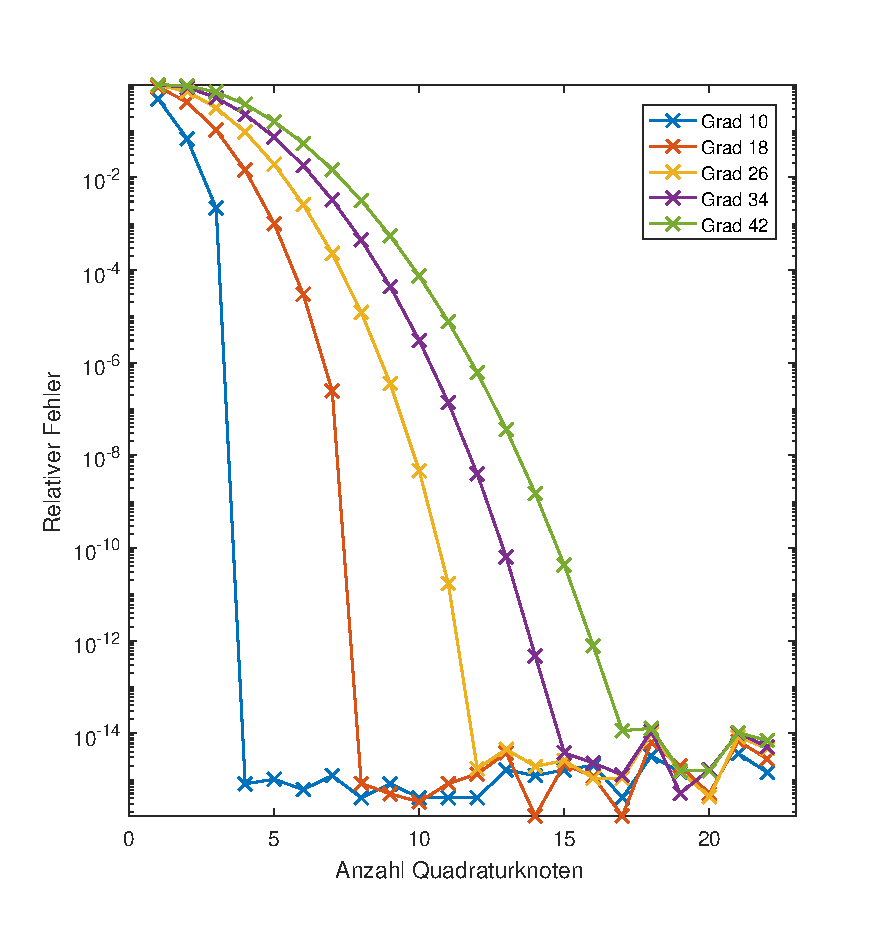
\includegraphics[width=0.9\linewidth]{Rel-Fehler-1D.eps}
	\caption{Vergleich relativer Fehler der Quadratur von Polynomen verschiedenen Grades über verschiedene Anzahl von Quadraturknoten.}
	\label{fig:relError1D}
\end{figure}

\begin{figure}[h]
	\centering
	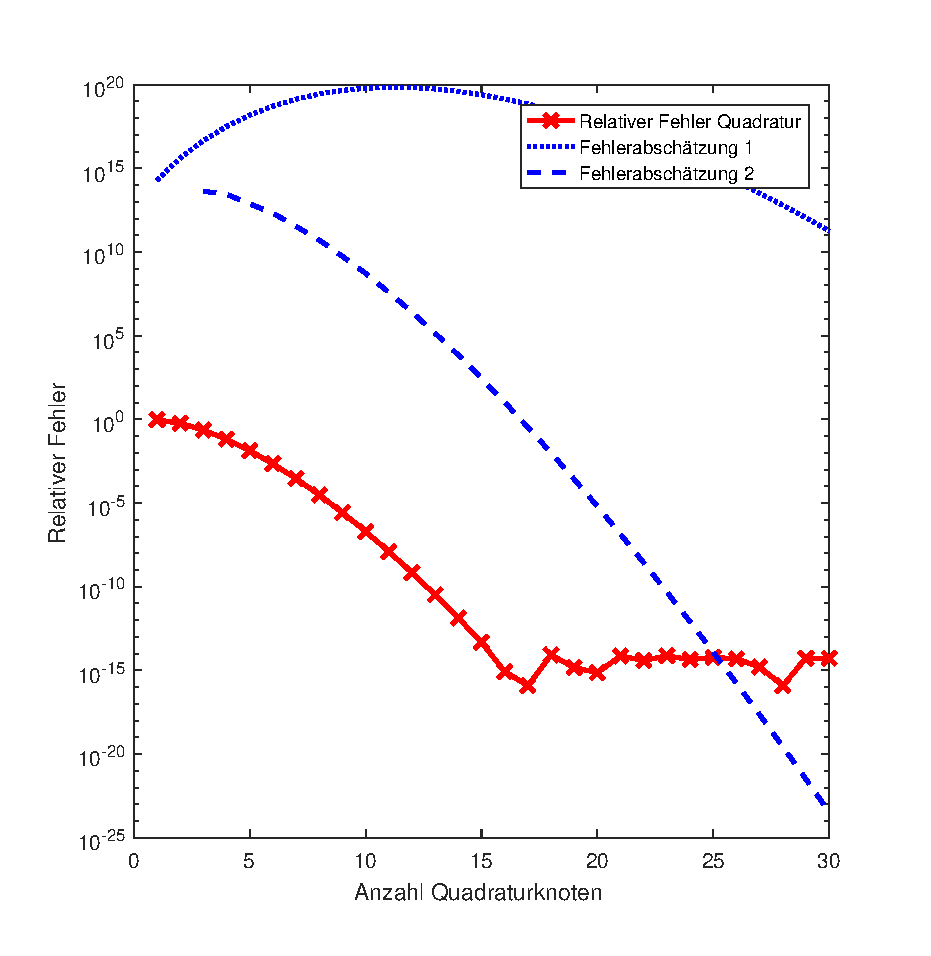
\includegraphics[width=0.9\linewidth]{Rel-Fehler-Exp.eps}
	\caption{Relativer Fehler der Quadratur $e^x$ verschiedene Anzahl von Quadraturknoten. Die Fehlerabschätzungen wurden durch ~\eqref{eq:apriori1} bzw ~\eqref{eq:apriori2} berechnet.}
	\label{fig:relError1DExp}
\end{figure}

\begin{figure}[h]
	\centering
	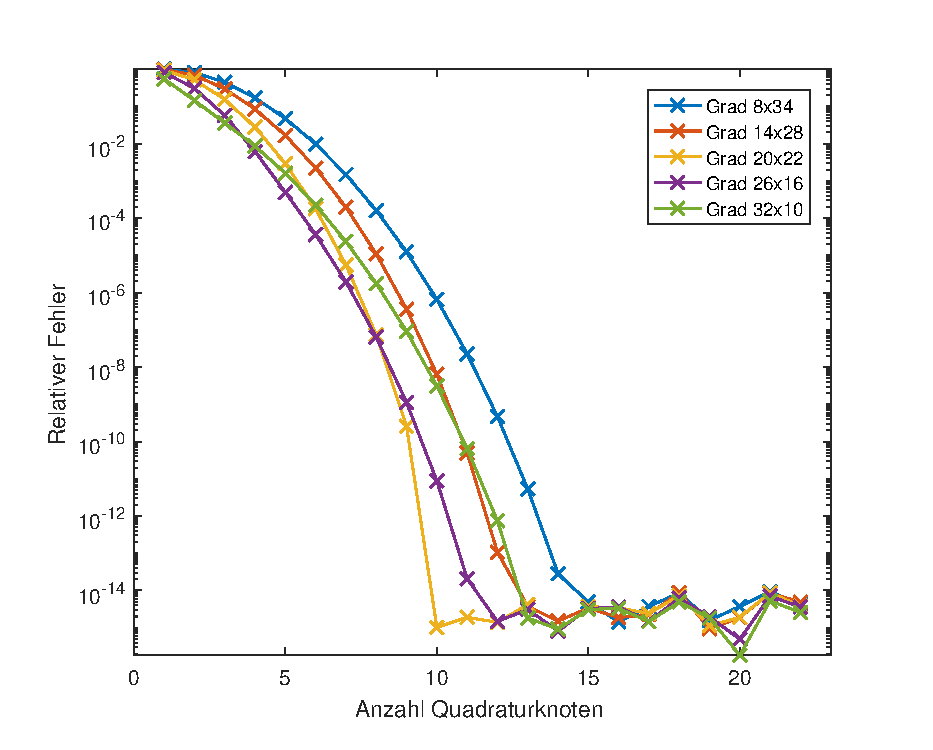
\includegraphics[width=0.9\linewidth]{Rel-Fehler-R.eps}
	\caption{Vergleich von relativen Fehler der Quadratur von Polynomen mit 2 Unbestimmten konstanten Grades auf $[0,1]^2$ über verschiedene Anzahl von Quadraturknoten.}
	\label{fig:relErrorR}
\end{figure}

\begin{figure}[h]
\centering
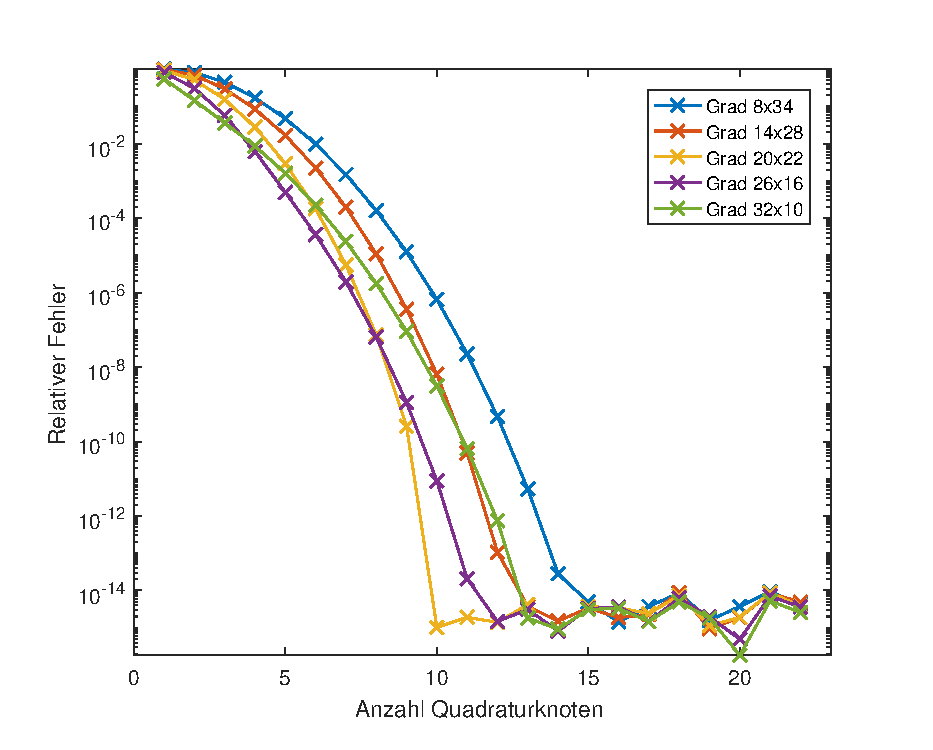
\includegraphics[width=0.9\linewidth]{Rel-Fehler-R.eps}
\caption{Vergleich von relativen Fehler der Quadratur von Polynomen mit 2 Unbestimmten verschiedenen Grades auf $\hat{T}$ über verschiedene Anzahl von Quadraturknoten.}
\label{fig:relErrort}
\end{figure}

\begin{figure}[h]
	\centering
	\begin{subfigure}[b]{0.7\textwidth}
		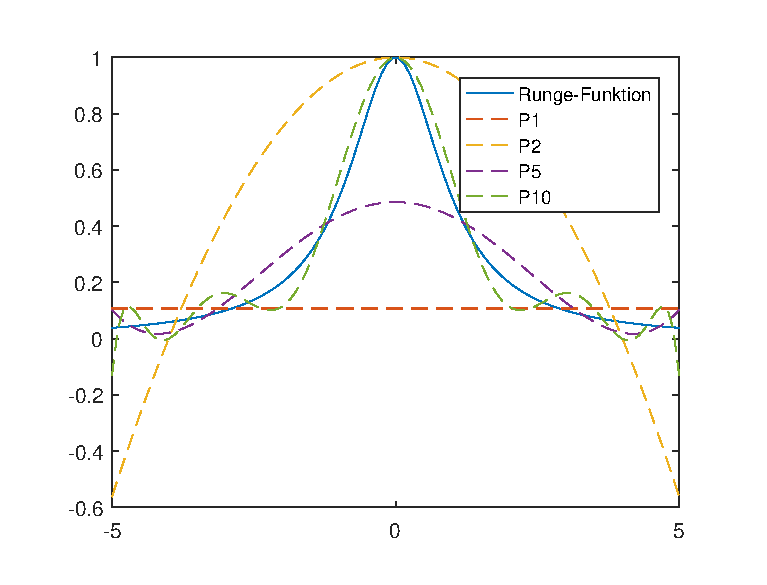
\includegraphics[width=1\linewidth]{Runge-fkt-poly.eps}
		\caption{Vergleich von Runge-Funktion und den Polynomen, die die implizit in der Gauß-Quadratur genutzt werden.}
		\label{fig:RungePoly}
	\end{subfigure}
	\begin{subfigure}[b]{0.7\textwidth}
		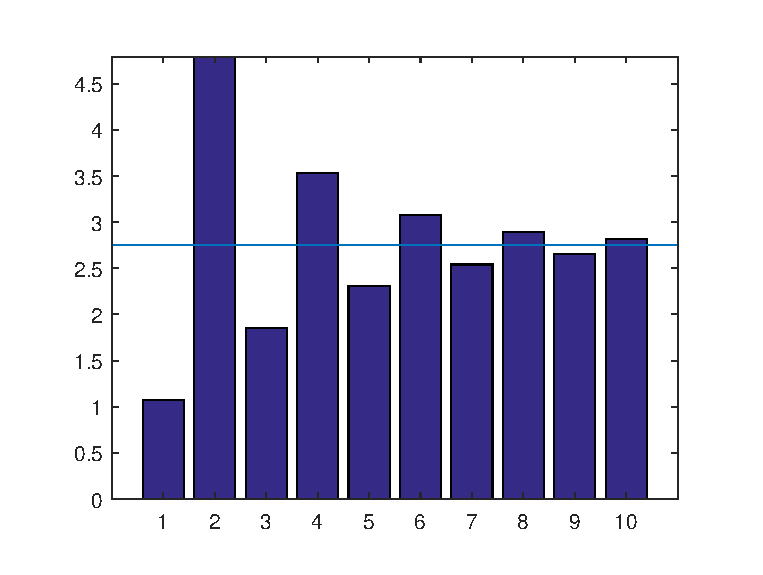
\includegraphics[width=1\linewidth]{Runge-fkt-Quadratur.eps}
		\caption{Vergleich der Werte der Quadratur Runge-Funktion, entsprechend der Anzahl der Quadraturknoten.}
		\label{fig:RungeQuadratur}
	\end{subfigure}
	\caption{Runge-Funktion und Interpolation}
	\label{fig:RungeFkt}
\end{figure}

\end{document}

%Version 1 (7.12.17) BK





